% This template is a generic paper template working with both the USENIX
% and ACM SIGPLAN and sig-alternate styles.
% It adds various conveniences and useful packages.
%
% Developed, munged and cluttered by Malte Schwarzkopf,
% University of Cambridge Computer Laboratory, 2009-2012.

% (Tested) options: sig-alternate, sig-alternate-10pt, article
% For USENIX template, use "article" and then add package "usenix"
% below.
\documentclass[letter,twocolumn,10pt]{sig-alternate-10pt}
%\documentclass[letterpaper,10pt]{article}
% Uncomment for USENIX style.
%\usepackage{usenix,epsfig} %,endnotes}
\usepackage{times}
% Don't fiddle with margins until explicitly requested!
%\usepackage[left=2cm,right=2cm,top=2cm,bottom=2cm]{geometry}

% Force paper size to letter (if necessary)
\usepackage[left=0.75in,right=0.75in,top=0.875in,bottom=0.875in,letterpaper]{geometry}
\setlength{\columnsep}{0.33in}

% Conditionals (for draft mode)
\usepackage{ifthen}

% Colro
\usepackage{color}

% Special fractions -- commented out as it doesn't work on Mac
%\usepackage{nicefrac}

% Symbols
\usepackage{textcomp}

% Outline package for rough notes
\usepackage{outlines}

% Bibliography
\usepackage[sort&compress,numbers]{natbib}

% TikZ figures
\usepackage{pgfplots}

% Buy us a little more space by allowing unindented enumerations
\usepackage{enumitem}

% Subfigures -- DEPRECATED, using subcaption instead
%\usepackage{subfig}

% Anil's magic
%\usepackage[compact]{titlesec}

% Balance columns
\usepackage{balance}

% Subfigures and captions
\usepackage{caption}
\usepackage{subcaption}

% Multi-row table cells
\usepackage{multirow}

% Landscape tables
\usepackage{rotating}

%Maths symbols
%\usepackage{mathtools}

% Date/time stuff
\usepackage{datetime}

% Tick/cross symbols
\usepackage{amsfonts}
\usepackage{amsmath}
\usepackage{pifont}

% Slanted fractions
\usepackage{xfrac}

%Code listings
%\usepackage{listings}      
%\usepackage{algorithm}% http://ctan.org/pkg/algorithms
%\usepackage[lined,boxed,commentsnumbered, linesnumbered]{algorithm2e}
\usepackage[lined,boxed,commentsnumbered]{algorithm2e}

%\usepackage{algpseudocode}% http://ctan.org/pkg/algorithmicx
       

%%%%%%%%%%%%%%%%%%%%%%%%%%%%%%%%%%%%%%%%%%%%%%%%%%%%%%%%%%%%%%%%%%%%%%%%%%%%%%%
% The BIG DRAFT SWITCH - Set to true to enable draft mode
%
% !!! This will produce extra output that
%     is not part of the final paper !!!

\newboolean{draft}
\setboolean{draft}{true}
%%%%%%%%%%%%%%%%%%%%%%%%%%%%%%%%%%%%%%%%%%%%%%%%%%%%%%%%%%%%%%%%%%%%%%%%%%%%%%%

\newcommand\note[2]{\ifdraft{\bf\color{#1}{\footnote{{\color{#1}\bf #2}}}\fi}}
\newcommand\ms[1]{{\note{blue}{Malte: #1}}}
\newcommand\mpg[1]{\note{orange}{Matt: #1}}
\newcommand\icg[1]{\note{purple}{Ionel: #1}}
\newcommand\awm[1]{\note{green}{AWM: #1}}

\newcommand\todo[1]{\ifdraft{\color{red}{\bf ToDo: #1}}\fi}

\newcommand\code[1]{\texttt{#1}}

% URL formatting
\usepackage{url}

% Multi-line comments
\usepackage{comment}

% Watermark in draft mode
% Draft watermark
\ifdraft
 \usepackage{graphicx}
 \usepackage{type1cm}
 \usepackage{eso-pic}
 \makeatletter
 \ddmmyyyydate
 \AddToShipoutPicture{%
             \setlength{\@tempdimb}{.5\paperwidth}%
             \setlength{\@tempdimc}{.5\paperheight}%
             \setlength{\unitlength}{1pt}%
             \put(\strip@pt\@tempdimb,\strip@pt\@tempdimc){%
         \makebox(0,700){\textcolor[gray]{0.50}%
%        {\fontsize{20pt}{20pt}\selectfont{Draft of \today{}, {\currenttime} -- please do not distribute.}}}%
         {\fontsize{20pt}{20pt}\selectfont{Under submission -- please do not distribute.}}}%
         \makebox(0,0){\rotatebox{45}{\textcolor[gray]{0.92}%
         {\fontsize{6cm}{6cm}\selectfont{DRAFT}}}}%
             }%
 }
\fi

% Mathcal hack
\DeclareMathAlphabet{\mathcal}{OMS}{cmsy}{m}{n}

% Enumeration commands
\newcommand{\one}{({\em i}\/)}
\newcommand{\two}{({\em ii}\/)}
\newcommand{\three}{({\em iii}\/)}
\newcommand{\four}{({\em iv}\/)}
\newcommand{\five}{({\em v}\/)}

% Symbol definitions
\newcommand{\tinydag}{\textsuperscript{\dag}}
\newcommand{\tinyddag}{\textsuperscript{\ddag}}
\newcommand{\tinystar}{\textsuperscript{$\ast$}}
\newcommand{\tick}{{\color{black}{\ding{51}}}}
\newcommand{\cross}{{\color{red}{\ding{55}}}}
\newcommand{\yes}{\ding{51}}
\newcommand{\no}{--}

% Various terms
\newcommand{\ciel}{\textsc{Ciel}}
\newcommand{\osconcept}{\textsc{Dios}}
\newcommand{\os}{D\textcent{}OS}
\newcommand{\system}{Q-Jump}
\newcommand{\systemshort}{QJ}
\newcommand{\llnet}{LLNet}
\newcommand{\bbnet}{BBNet}

% Helpful time shortcuts
\newcommand{\millis}{$\mathrm{ms}$}
\newcommand{\micros}{$\mu\mathrm{s}$}
\newcommand{\nanos}{$\mathrm{ns}$}

% "th" superscript
\newcommand{\thss}{\textsuperscript{th}}

% Fancy math mode typesetting
\newcommand\scref[1]{$\mathcal{R}_#1$}

% italicize figure captions
\usepackage{caption}
\renewcommand{\captionfont}{\itshape}

% Macros for structural work in early stages
\newcommand\figdesc[4]{\framebox[\columnwidth]{\small\centering\parbox{0.95\columnwidth}{\textbf{Type:} #1\par \textbf{$x$-axis:} #2\par \textbf{$y$-axis:} #3\par \textbf{Message:} #4}}}

\begin{document}

% SIG templates only (!!!)
% --- Author Metadata here ---
\conferenceinfo{SIGCOMM}{2014, Chicago, IL, USA}
%\CopyrightYear{2007} % Allows default copyright year (20XX) to be over-ridden - IF NEED BE.
%\crdata{0-12345-67-8/90/01}  % Allows default copyright data (0-89791-88-6/97/05) to be over-ridden - IF NEED BE.
% --- End of Author Metadata ---

%don't want date printed
%\date{}

%\title{\system{}: Eliminating Interference in\\ Your Data Center Network}
\title{ Decompressing TCP/IP Headers for High-Speed Links \\ (or How to Build a 100Gb/s Network Stack)}

% Number of authors
\numberofauthors{1}

% Authors
\author{
% First
\alignauthor
Under submission for review.
%Smart people \\
%  \affaddr{University of Cambridge Computer Laboratory}\\
%  \email{\url{first.last@cl.cam.ac.uk}}
}

\maketitle

%\preprintfooter{Version of {\currenttime}, \today.}

% Use the following at camera-ready time to suppress page numbers.
% Comment it out when you first submit the paper for review.
%\pagestyle{empty}

%%%%%%%%%%%%%%%%%%%%%%%%%%%%%%%%%%%%%%%%%%%%%%%%%%%%%%%%%%%%%%%%%%%%%%%%%%%%
% ABSTRACT
%%%%%%%%%%%%%%%%%%%%%%%%%%%%%%%%%%%%%%%%%%%%%%%%%%%%%%%%%%%%%%%%%%%%%%%%%%%%

\begin{abstract}

%Making a conscious effort to remove "britishisms" from the text -- thus, hence, whilst, while, yet, whereas, etc. 
%Also trying to slim down on adjectives. One mans's "very" is another man's "some". 
%To make diff/merge easier. I am now putting 1 "statement" (sentence) per line. 
%Trying to apply the KISS principle, especially to the language used, to help out our American reviewers. 


% What is the problem?
Network protocol implementations are stuck in the 1980s. Bits and bytes are squeezed next to each other to maximise efficiency for slow link speeds and fast CPUs. However, CPU speeds have plateaued for several years and network speeds have increased rapidly. 
%40Gb/s NICs are now commodity and 100Gb/s devices are entering the market. 
% Why does it matter?
Single CPU cores can no longer hope to keep up with doing per-packet network encoding and decoding. 
%, especially when bits and bytes are in such plentiful supply on the wire.

% What is our solution?
%In opposition to Van Jacobson's classic RFC 1144 ``\emph{Compressing TCP/IP Headers for Low-Speed Serial Links}'', we propose 
We investigate several options for expanding, aligning, and sizing TCP/IP\ms{We don't really do TCP...} and Ethernet packets to maximise efficiency for our (now) slow, 64-bit, little-endian, CPUs.  
% Why is it good?
In these first steps toward a practical, high speed network stack, we show that combining Direct Cache Access (DCA)\ms{Do we have any numbers on this?} with real zero-copy delivery and restructured 64-bit alignment of packet fields are crucial to packet processing beyond 40Gb/s. Further, we demonstrate a simple user-space network stack capable of handling over 100Gb/s of traffic on a single core and maintaining up to 100Gb/s per core over multiple cores.


\end{abstract}


%%%%%%%%%%%%%%%%%%%%%%%%%%%%%%%%%%%%%%%%%%%%%%%%%%%%%%%%%%%%%%%%%%%%%%%%%%%%
% CONTENT SECTION INCLUDES
%%%%%%%%%%%%%%%%%%%%%%%%%%%%%%%%%%%%%%%%%%%%%%%%%%%%%%%%%%%%%%%%%%%%%%%%%%%%

%%%%%%%%%%%%%%%%%%%%%%%%%%%%%%%%%%%%%%%%%%%%%%%%%%%%%%%%%%%%%%%%%%%%%%%%%%%
% 1) INTRO
%%%%%%%%%%%%%%%%%%%%%%%%%%%%%%%%%%%%%%%%%%%%%%%%%%%%%%%%%%%%%%%%%%%%%%%%%%%

\section{Introduction}
\label{s:intro}

%Making a conscious effort to remove "britishisms" from the text -- thus, hence, whilst, while, yet, whereas, etc. 
%Also trying to slim down on adjectives. One mans's "very" is another man's "some". 
%To make diff/merge easier. I am now putting 1 "statement" (sentence) per line. 
%Trying to apply the KISS principle, especially to the language used, to help out our American reviewers. 

By classical wisdom, smaller packet headers are better: fewer bits wasted on the wire mean greater efficiency overall. 
Van Jacobson's impressive RFC~1144~\cite{rfc1144} ``\emph{Compressing TCP/IP Headers for Low-Speed Serial Links}'' takes this concept to the extreme.
It shows how to compress the 40 byte TCP/IP header down to less than 4 bytes in the common case. 


Despite the heroic efforts of Jacobson and others to keep TCP/IP headers short, saving bits on the wire is only beneficial if the cost of transmission outweighs the cost of compression. 
For example, on a 9600b/s serial link, each bit costs around 10 microseconds to transmit. 
By saving 36 bytes per packet, Jacobson could save just under 30 milliseconds per transmission.
From a total round trip budget of 100 milliseconds, 30 milliseconds represented an impressive saving.


On a modern 40Gb/s Ethernet link, each bit now costs 25 picoseconds to transmit.
A best-in-class CPU running at 4GHz executes only one cycle every 250 picoseconds. 
This means that the CPU needs to be able to process an average of 10 bits per cycle to keep up with line-rate. 
As we go forward, power and thermal efficiency issues are causing CPUs to get slower and wider rather than faster. 
Intel's new Haswell CPUs typically execute 1 cycle every 500 picoseconds (2GHz). 
By contrast, networks are getting faster. A 100Gb/s Ethernet link can transmit 1 bit every 10 picoseconds, a factor of 50x faster. 
This means that CPUs now need to process on average 50 bits per cycle just to keep up. 
%This leaves no time for handling anything other than packet processing. 


A 64-bit CPU should be able to cope with 64 bits per cycle, as long as each instruction requires only one cycle. % and it operates on the whole 64 bits at once.
Modern CPUs typically require multiple cycles for many instructions.
By packing bits tightly together and by aligning fields on 16-bit (Ethernet) or 32-bit (TCP/IP) boundaries, we guarantee that the CPU will need to do more than 1 instruction per header field. 


\begin{figure}
 \centering
 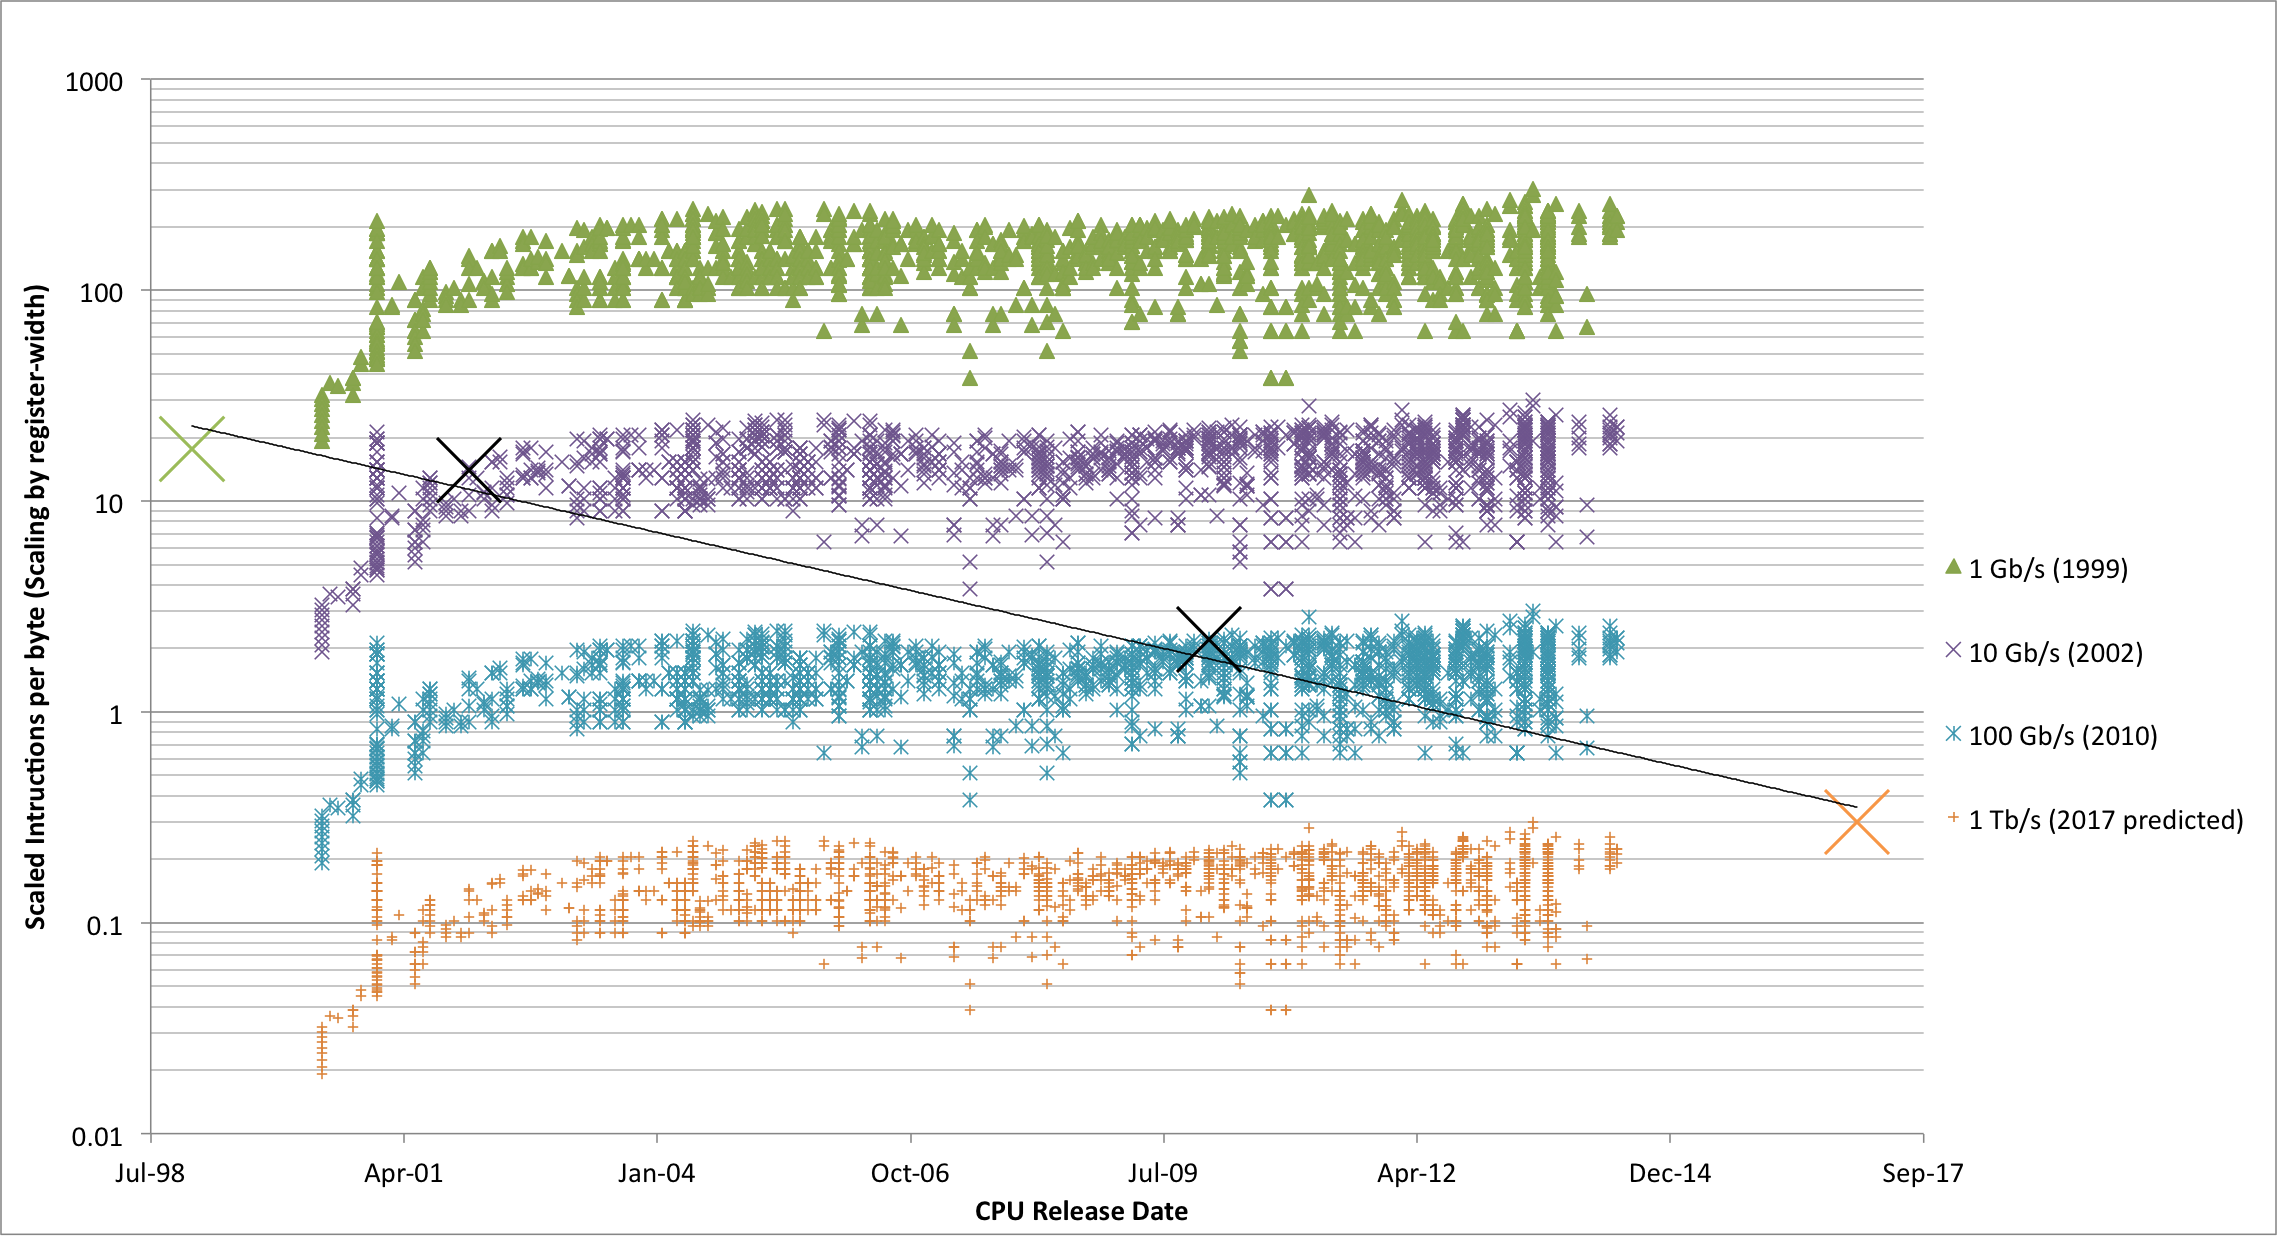
\includegraphics[width=1\columnwidth]{figures/cpu/ips-figure.png}
 \caption{Instructions per network-byte for a range of Ethernet technologies. Despite scaling by instruction width, the flattening of CPU instruction-rate is clear.  }
 \label{f:ips-figure}
\end{figure}



It gets worse. 
Network packets are transmitted using network byte ordering which is "big-endian", but the majority of CPUs today use "little-endian" byte ordering internally. 
Once the CPU has found and extracted the correct field from a packet, it then needs to reorder the bytes into little-endian format. % before it can do anything useful with them. 
The little-endian conversion adds strain to an already tight cycle budget.


From these examples, it should be clear that CPU cycles are becoming a rare commodity and that network bits are now plentiful. We think that the time has come to reevaluate the tradeoffs in on-the-wire formats for TCP/IP protocols. 
Specifically, we consider if there are optimisations to the layout of packets in host memory only, without changing the functionality of the protocols themselves. 
To do this, we build a simple network stack that runs directly out of host memory. 
We then test a variety of different packet layouts and show that gains of nearly 3$\times{}$ can be found by arranging packet wire formats correctly, allowing network stacks to scale beyond 40Gb/s and up to over 100Gb/s. 


%Ultimately we show how to build a simple network stack, capable of processing above 100Gb/s on a single core. 
%By applying optimisations to this stack, we can test the limits of CPU based network processing. Since our stack in minimal and our CPU is fast, our experiments represent the absolute limit. Our "application" emulation simply reads intergers out of the packet in an array and in


%For an intuitive sense of the problem, consider a 

%
%We consider the following questions: 
%- Can expanding the number of bits assigned to a given field reduce the overall processing time, despite a modest increase in the transmission time. 
%- Is the big endian “network” byte order costing more than it benefits considering that the majority of machines in operation are little endian.
%- Is it necessary that packet layout reflects layering found in the protocol stack, or are there optimisations to be found by rearranging packet contents. 
%- Can these optimisations be made transparently to the network legacy network stack in much the same way that Van Jacobson achieved header compression. 
%
%Evaluation Proposal: 
%- Instrument linux (and? BSD) stack - Count the cycles it takes to process UDP/TCP/ICMP/ARP - Count the min/max/med/ave/std-dev cycles per bit. 
%- Build a simple UDP/ICMP/ARP (maybe using Netmap or DPDK) that is faster than Linux. 
%- Since our stack is faster than linux, it must necessarily be doing less work per bit. Count the min/max/med/ave/std-dev cycles per bit. 
%- Show that we can do even less work (cycles and/or instructions) by expanding the headers. Compare the Count the min/max/med/ave/std-dev cycles per bit. to above. 
%
%(Maybe do this for both ipv4 and ipv6) 
%
%Conclude that we can make cycles per bit go down by expanding headers, and predict what this will mean for near future cpu architectures/very high link speeds. 

%%%%%%%%%%%%%%%%%%%%%%%%%%%%%%%%%%%%%%%%%%%%%%%%%%%%%%%%%%%%%%%%%%%%%%%%%%%
% 2) Experimental Setup
%%%%%%%%%%%%%%%%%%%%%%%%%%%%%%%%%%%%%%%%%%%%%%%%%%%%%%%%%%%%%%%%%%%%%%%%%%%

%Making a conscious effort to remove "britishisms" from the text -- thus, hence, whilst, while, yet, furthermore, whereas, etc. 
%Also trying to slim down on adjectives. One mans's "very" is another man's "some". 
%To make diff/merge easier. I am now putting 1 "statement" (sentence) per line. 
%Trying to apply the KISS principle, especially to the language used, to help out our American reviewers. 

\begin{algorithm}

 \SetKw{To}{to}
 \SetKw{StartTimer}{start $\leftarrow$ timer}
 \SetKw{StopTimer}{stop $\leftarrow$ timer}
 \SetKw{Continue}{continue}
 \ForEach{ packet in packet\_buffer }{
    \BlankLine          
     \StartTimer{}\;
     \BlankLine
     packet.ethernet.src $\leftarrow$ 0xFFFFFF\; 
     packet.ethernet.dst $\leftarrow$ 0x000001\;
     packet.ethernet.type $\leftarrow$ 0x0800\; 
     $\cdots$\\     
     packet.ip.size $\leftarrow$ \emph{big\_endian}(IP\_SIZE)\;
     $\cdots$\\     
     packet.ip.protocol $\leftarrow$  0x11\;
     $\cdots$\\         
     packet.udp.size $\leftarrow$ \emph{big\_endian}(UDP\_SIZE)\;          
     $\cdots$\\
     \For{ i $\leftarrow$ 0 \To{} UDP\_SIZE $\div{}$ WORD\_SIZE}{
         packet.udp.data[\emph{i}] $\leftarrow$ const integer\;
     }
     \BlankLine
     \StopTimer{}\;
     \BlankLine
 }


\caption{Generating packets}
\label{alg:net_gen}
\end{algorithm}


\section{Testing High Speed Networks}
\label{s:experiments}
To test the effect of packet layouts on processing speed, we would like to use a flexible, high speed network adapter. 
Some FPGA based 100Gb/s network adapters are beginning to appear on the market~\cite{100gnic}, but they are rare and expensive. 
Additionally, adapting 1000's of lines of legacy network stack code to process new packet formats will be time consuming. 
To work around these problems, we take a different approach. 
Instead of building a network stack for a particular adapter, we use our experience in high speed network adapter design \emph{[reference removed for blind review]} to build a generic network stack that runs directly out of system memory. 
We assume that an adapter will eventually become available to place packets there. 
This allows us to test the absolute speed of packet processing quickly and flexibly 
It also gives us an indication of the expected upper limits that software could expect to achieve. 
By writing our own network stack, we free ourselves from legacy code bases and can ensure that our packet processor is flexible enough to cope with a range of different packet formats. 


Our initial network stack only processes UDP packets, delivered over IP version 4.0 transport using Ethernet frames. 
In principle any protocol or transport could be supported, but this is the simplest to implement. 
By doing so, we can get a strong indication of the practical upper bounds of any reasonable network stack. 


Our network stack is divided into two parts: generating and receiving packets. 
Packet generation is detailed in Algorithm~\ref{alg:net_gen} and packet receiving is detailed in Algorithm~\ref{alg:net_rcv}. 
For each experiment, we first run the generation phase and then the receiving phase. This way we can test both parts independently. 
As with any sensible network stack, we only perform endian conversions for values that are non-constant. 
For example, the ethernet packet type field is a constant, but the IP header size is not. 
Our packet buffer is pinned so that swapping cannot happen and aligned to a 4kB page boundary. 

Our experiments are run using a top-of-the range Intel Core i7 Ivy Bridge CPU (4930K), with 12 threads running at 3.4GHz. 
We ensure that the network-stack process is pinned to a unique CPU, with no other processes or hyperthreads interfering and that the process is run with full-realtime priority. 
This environment is overly generous. 
Real in-kernel network stacks have limited time to run and have to contend with interrupts and threads from other competing resources. 




\begin{algorithm}
 \SetKw{Continue}{continue}
 \SetKw{To}{to}
 \SetKw{StartTimer}{start $\leftarrow$ timer}
 \SetKw{StopTimer}{stop $\leftarrow$ timer}

 \ForEach{ packet in packet\_buffer }{
     \BlankLine
     \StartTimer{}\;
     \BlankLine
     \If{ packet.ethernet.src $\neq$ 0xFFFFFF }{
        \Continue{};
     }
     \If{ packet.ethernet.dst $\neq$ 0x000001 }{
        \Continue{};
     }
     \If{ packet.ethernet.type $\neq$  0x0800 }{
        \Continue{};
     }
     $\cdots$\\
     ip\_size $\leftarrow$ \emph{little\_endian}(packet.ip.size)\;
     total\_ip\_bytes $\leftarrow$ total\_ip\_bytes + ip\_size\;
     $\cdots$\\     
      \If{ packet.ip.protocol $\neq$  0x11 }{
        \Continue{}\;
     }
     $\cdots$\\         
     udp\_size $\leftarrow$ \emph{little\_endian}(packet.udp.size)\;     
     total\_udp\_bytes $\leftarrow$ total\_udp\_bytes + udp\_size\;     
     $\cdots$\\
     counter $\leftarrow$ 0\;
     \For{ i $\leftarrow$ 0 \To{} udp\_size $\div{}$ WORD\_SIZE}{
         counter $\leftarrow$ packet.udp.data[\emph{i}];
     }
     \BlankLine
     \StopTimer{}\;    
     \BlankLine
     
 }

\caption{Receiving packets}
\label{alg:net_rcv}
\end{algorithm}


%%%%%%%%%%%%%%%%%%%%%%%%%%%%%%%%%%%%%%%%%%%%%%%%%%%%%%%%%%%%%%%%%%%%%%%%%%%
% 3) Evaluation
%%%%%%%%%%%%%%%%%%%%%%%%%%%%%%%%%%%%%%%%%%%%%%%%%%%%%%%%%%%%%%%%%%%%%%%%%%%

\section{Evaluation}
\subsection{Baseline}
Discuss the current performance speeds with packet layouts how they are. 

\subsection{Memory speed}

Show how zero copy and memory allocation (eg DCA) affect the overall performance. 

\subsection{Network Byte Ordering}

Show how network byte ordering affects the speed. 

\subsection{Packet layouts}

Show how network byte ordering affects the speed. 

\subsection{Core Scaling}

Show how this scales as we increase core counts.

%%%%%%%%%%%%%%%%%%%%%%%%%%%%%%%%%%%%%%%%%%%%%%%%%%%%%%%%%%%%%%%%%%%%%%%%%%%
% 3) Evaluation
%%%%%%%%%%%%%%%%%%%%%%%%%%%%%%%%%%%%%%%%%%%%%%%%%%%%%%%%%%%%%%%%%%%%%%%%%%%

\section{Discussion}

%%%%%%%%%%%%%%%%%%%%%%%%%%%%%%%%%%%%%%%%%%%%%%%%%%%%%%%%%%%%%%%%%%%%%%%%%%%
% 3) Evaluation
%%%%%%%%%%%%%%%%%%%%%%%%%%%%%%%%%%%%%%%%%%%%%%%%%%%%%%%%%%%%%%%%%%%%%%%%%%%

\section{Related Work}

\todo{AWM comments:}
\begin{enumerate}
 \item \emph{isn't this all solved by hardware offload stuff?} -- not sure what the answer is there\ms{a NIC could potentially DMA larger, better-aligned frames, but that would be wasteful of bus bandwidht...}
 \item \emph{but my machine has lots of cores...} -- not helpful, since packet decoding is unsplittable and cannot be parallelised. Even a single TCP flow cannot be parallelised over multiple cores.
\end{enumerate}


The penetration of hardware offload features promotes a belief that we have solved the mismatch between network speed and host capacity. However, beyond the most rudimentary offload --- those plausible on a packet-by-packet basis: checksum offload, packetization and packet aggregation --- offload has not proven to be widely useful.\ms{why?} Mogul~\cite{mogul2003tcp} provided a sober insight into this by noting that best-use offload was in extremely specialised circumstance: the per-application networking including per-application offload engines. However, in opposition to this networking continues to be the provenance of the operating system: providing a generic service to every application. Thus providing limited ability to specialise tasks for specific hardware.
\awm{jibberish written by a tired brain}


%%%%%%%%%%%%%%%%%%%%%%%%%%%%%%%%%%%%%%%%%%%%%%%%%%%%%%%%%%%%%%%%%%%%%%%%%%%
% 3) Evaluation
%%%%%%%%%%%%%%%%%%%%%%%%%%%%%%%%%%%%%%%%%%%%%%%%%%%%%%%%%%%%%%%%%%%%%%%%%%%

\section{Conclusions}




%%%%%%%%%%%%%%%%%%%%%%%%%%%%%%%%%%%%%%%%%%%%%%%%%%%%%%%%%%%%%%%%%%%%%%%%%%%%
% BIBLIOGRAPHY
%%%%%%%%%%%%%%%%%%%%%%%%%%%%%%%%%%%%%%%%%%%%%%%%%%%%%%%%%%%%%%%%%%%%%%%%%%%%

{
\small
\setlength\bibsep{0.09em}
\balance
\bibliographystyle{acm}
\bibliography{local,r2d2,phdreferences,rfc}

}

% \theendnotes

\end{document}
